\documentclass[tikz,border=8pt]{standalone}
% Shared look for every TikZ diagram. Load with \input{../../tools/tikz-style.tex}
\usepackage[T1]{fontenc}
\usepackage{lmodern}
\renewcommand{\sfdefault}{lmr}  % diagrams use the same serif as the text
\usetikzlibrary{arrows.meta, positioning, shapes.geometric, calc, fit, backgrounds}
\definecolor{cblue}{HTML}{4C78A8}
\definecolor{corange}{HTML}{F58518}
\definecolor{cgreen}{HTML}{54A24B}
\definecolor{cred}{HTML}{E45756}
\definecolor{cpurple}{HTML}{B279A2}
\definecolor{cgrey}{HTML}{6B6B6B}
\tikzset{
  every picture/.style={font=\sffamily, line width=1.2pt},
  box/.style={draw=#1, fill=#1!12, rounded corners=4pt, align=center, inner sep=7pt, minimum height=1.1cm},
  box/.default=cgrey,
  arrow/.style={-{Stealth[length=3mm]}, draw=cgrey, line width=1.4pt},
  title/.style={font=\sffamily\bfseries\Large},
  note/.style={font=\sffamily\small, text=cgrey, align=center},
}
\AtBeginDocument{\hyphenpenalty=10000 \exhyphenpenalty=10000}

\begin{document}
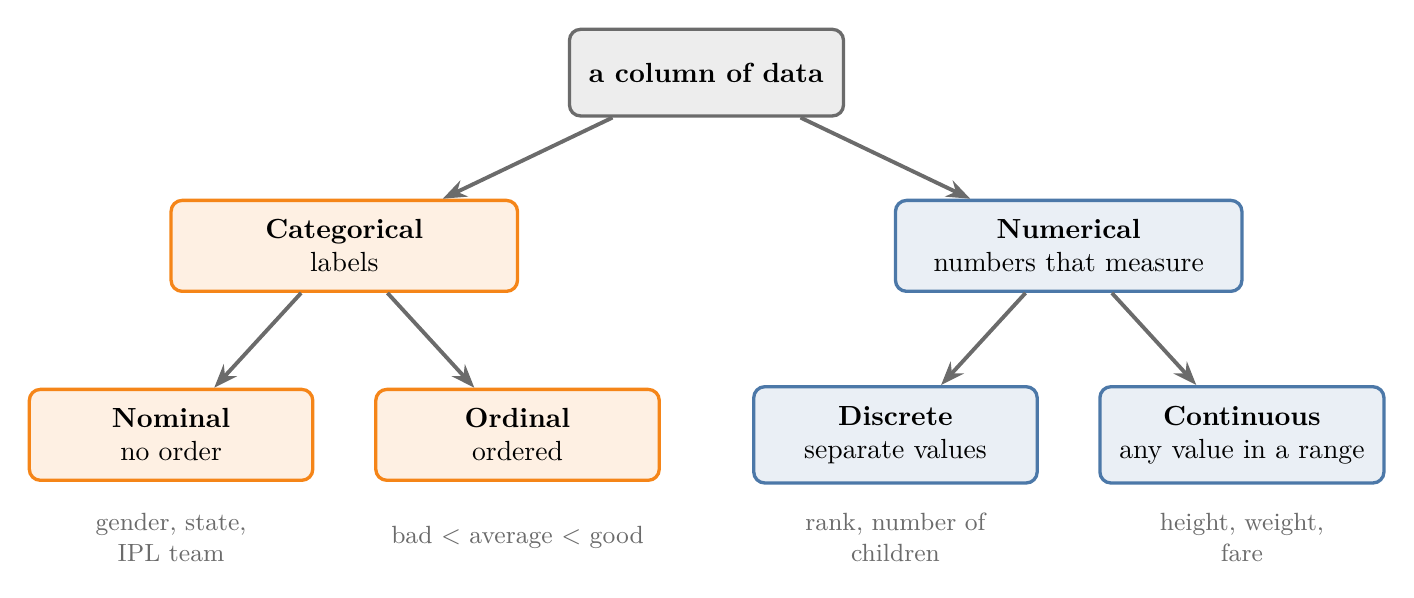
\begin{tikzpicture}[level distance=2.3cm, sibling distance=4.4cm]
  \node[box] (d) at (0,0) {\textbf{a column of data}};
  \node[box=corange, minimum width=4.4cm] (c) at (-4.6,-2.2) {\textbf{Categorical}\\ labels};
  \node[box=cblue, minimum width=4.4cm] (n) at (4.6,-2.2) {\textbf{Numerical}\\ numbers that measure};
  \node[box=corange, minimum width=3.6cm] (nom) at (-6.8,-4.6) {\textbf{Nominal}\\ no order};
  \node[box=corange, minimum width=3.6cm] (ord) at (-2.4,-4.6) {\textbf{Ordinal}\\ ordered};
  \node[box=cblue, minimum width=3.6cm] (dis) at (2.4,-4.6) {\textbf{Discrete}\\ separate values};
  \node[box=cblue, minimum width=3.6cm] (con) at (6.8,-4.6) {\textbf{Continuous}\\ any value in a range};
  \foreach \a/\b in {d/c, d/n, c/nom, c/ord, n/dis, n/con} \draw[arrow] (\a) -- (\b);
  \node[note] at (-6.8,-5.9) {gender, state,\\ IPL team};
  \node[note] at (-2.4,-5.9) {bad $<$ average $<$ good};
  \node[note] at (2.4,-5.9) {rank, number of\\ children};
  \node[note] at (6.8,-5.9) {height, weight,\\ fare};
\end{tikzpicture}
\end{document}
